\documentclass[10pt,twocolumn]{article}
\usepackage[margin=0.6in]{geometry}
\usepackage[T1]{fontenc}
\usepackage[utf8]{inputenc}
\usepackage{lmodern}
\usepackage{amsmath}
\usepackage{graphicx}
\usepackage{booktabs}
\usepackage{array}
\usepackage{tabularx}
\usepackage[table]{xcolor}
\usepackage{enumitem}
\usepackage{caption}
\usepackage{tikz}
\usepackage{float}
\usepackage{placeins}
\usepackage{url}
\usepackage[hidelinks]{hyperref}
\usetikzlibrary{arrows.meta,positioning,calc}

\captionsetup{font=footnotesize,labelfont=bf}
\setlength{\columnsep}{0.20in}
\setlength{\parindent}{0pt}
\setlength{\parskip}{0.32em}
\raggedbottom

\title{\vspace{-1.5em}\textbf{Question Answering with a Custom Transformer Encoder and Generative Decoder}\vspace{-0.5em}}
\author{\href{https://github.com/Harsha081459/Question-Answer-System-with-a-Custom-Transformer-Encoder-and-Generative-Decoder}{\textbf{[GitHub]}} \quad $\mid$ \quad \href{https://iiitbac-my.sharepoint.com/:f:/g/personal/vishal_sriram_iiitb_ac_in/IgBJMBmHEodfQba6fYpup9aiAdhsUH577v5oWa_W0i20VqM?e=j7DCc6}
{\textbf{[Weights -- OneDrive]}} \quad $\mid$ \quad \href{https://huggingface.co/spaces/hv-123/QA-Engine}{\textbf{[Web App]}}}

\date{}

\begin{document}
\maketitle
\vspace{-2.5em}

% ── Team Information ──
\begin{table}[H]
\centering
\small
\caption*{\textbf{NLP (AID 829) --- Group Assignment $\mid$ Group 18}}
\vspace{-0.5em}
\begin{tabular}{@{}clc@{}}
\toprule
\textbf{S.No.} & \textbf{Name} & \textbf{Roll Number} \\
\midrule
1 & Vishal Sriram & BT2024036 \\
2 & Harsha & BT2024106 \\
3 & Lohith & BT2024248 \\
4 & Munjikesh & BT2024247 \\
\bottomrule
\end{tabular}
\end{table}
\vspace{-0.5em}

% ══════════════════════════════════════════════════════════════
\begin{abstract}
We built a SQuAD-based question answering system featuring two parallel tracks: an extractive span predictor and a custom generative answer decoder. Both tracks share a custom 12-layer Transformer encoder pretrained from scratch via masked language modeling. The extractive model was benchmarked against strong public baselines, confirming that our scratch-built encoder learns a competitive span-selection representation. For the generative track, we developed a bespoke 4-layer decoder optimized for concise answer generation. Evaluated on a shared validation subset, our custom decoder outperformed T5-small and Flan-T5-small, closely approaching T5-base.
\end{abstract}

% ══════════════════════════════════════════════════════════════
\section{Introduction}
Machine reading comprehension requires a model to process a question and context passage, then return a precise answer. This project addressed the task through two distinct modes: \textbf{extractive QA} (predicting start and end token indices of the answer span) and \textbf{generative QA} (decoding a short answer token-by-token from the encoder states). Implementing both modes provided a rigorous test of the underlying encoder's representational capacity.

The pipeline executed in four sequential stages:
\begin{enumerate}[leftmargin=1.2em,itemsep=3pt,topsep=4pt]
    \item \textbf{Stage 1:} Pretrain a BERT-style encoder from scratch using masked language modeling on Wikipedia + C4.
    \item \textbf{Stage 2:} Fine-tune the encoder for extractive QA on SQuAD v2.
    \item \textbf{Stage 3:} Construct a generative encoder-decoder on top of the same encoder.
    \item \textbf{Stage 4:} Expose both inference paths through a unified local demo.
\end{enumerate}

\vfill\columnbreak

\textbf{Primary contribution.} A clear engineering and research progression: a single custom-trained encoder powering both accurate extractive span prediction and competitive generative answer decoding without relying on off-the-shelf pretrained architectures.

% ══════════════════════════════════════════════════════════════
\section{Related Work}
Extractive QA was revolutionized by BERT \cite{devlin2019bert}, which introduced bidirectional Transformer pretraining via masked language modeling. Our encoder architecture closely follows the BERT-base specification: a 12-layer Transformer stack with 768-dimensional hidden states. While robustly optimized variants like RoBERTa \cite{liu2019roberta} achieve higher absolute performance on SQuAD \cite{rajpurkar2016squad}, our project focused on the pedagogical value of pretraining this architecture from scratch.

In generative QA, unified text-to-text Transformers like T5 \cite{raffel2020t5} dominate. We use T5-small and T5-base as external benchmarks, but our approach differs by grafting a lighter, bespoke 4-layer decoder onto our BERT-style encoder via a linear projection bridge. This hybrid design allowed strict control over decoding heuristics without inheriting the broad generation priors of massively pretrained seq2seq models.

% ══════════════════════════════════════════════════════════════
\section{System Architecture}

The system was designed around a single shared encoder whose contextual
representations power two structurally distinct inference heads. This
unified backbone architecture reflects a deliberate engineering choice:
rather than training separate models for extractive and generative QA,
we exploit the fact that both tasks require the same fundamental
capability --- grounding token-level representations in the joint
context of a question and a supporting passage.

\subsection{Input Representation}
Both inference paths begin with identical preprocessing. The question
and context are concatenated using the standard BERT-style
\texttt{[CLS] Q [SEP] C [SEP]} template. Three embedding matrices are
summed to form the initial token representation: a token embedding
($|\mathcal{V}| \times 768$), a learned positional embedding (up to
512 positions), and a segment embedding that distinguishes question
tokens (type~0) from context tokens (type~1). The summed embeddings
are passed through layer normalization and dropout before entering the
encoder stack.

\subsection{Shared Transformer Encoder}
The encoder is a 12-layer bidirectional Transformer. Each layer
applies pre-layer-norm multi-head self-attention (12 heads,
$d_k = d_v = 64$) followed by a two-layer feed-forward network with
hidden dimension 3072 and GELU activation. Residual connections wrap
both sub-layers. The full sequence output
$\mathbf{H} \in \mathbb{R}^{L \times 768}$ is passed to both
downstream heads, where $L$ is the padded sequence length (capped
at 256 tokens with a doc stride of 64 for long contexts).

The pre-norm variant was chosen over the original post-norm BERT
design because it yields more stable gradients during fine-tuning,
particularly when the encoder is jointly optimized with the decoder
at a lower learning rate.

\subsection{Extractive Head}
The extractive head is a single linear projection
$\mathbf{W} \in \mathbb{R}^{768 \times 2}$ applied independently to
every encoder output token. This produces two scalar logits per
position: $s_i$ (start score) and $e_i$ (end score). At inference
time, the top-$n_{\text{best}}$ start positions are enumerated and
paired with all legal end positions to form candidate spans. Each span is scored by summing its start and end logits, and the highest-scoring valid
span is returned as the extracted answer. For unanswerable questions
(SQuAD v2 no-answer instances), the score of the \texttt{[CLS]} token
logit serves as the null-answer score; if it exceeds the best span
score by a tuned threshold $\tau$, the model abstains.

\subsection{Encoder--Decoder Bridge}
Because the encoder operates in a 768-dimensional space while the
decoder uses a 512-dimensional space, a learned linear projection
$\mathbf{W}_{\text{bridge}} \in \mathbb{R}^{768 \times 512}$ maps
the full encoder memory $\mathbf{H}$ into the decoder's key--value
space before each cross-attention layer. This projection is trained
jointly with the decoder and allows the two modules to operate at
different widths without any information bottleneck beyond what
the linear map can express.

\subsection{Generative Decoder}
The generative decoder is a 4-layer autoregressive Transformer with
hidden dimension 512 and 8 attention heads ($d_k = d_v = 64$). Each
decoder block applies three sub-layers in sequence, each wrapped in a
pre-norm residual:

\begin{enumerate}[leftmargin=1.2em,noitemsep,topsep=2pt]
    \item \textbf{Masked self-attention.} Attends over all previously
    generated tokens using a causal mask, building up a
    representation of the partial answer prefix.
    \item \textbf{Cross-attention.} Queries the projected encoder
    memory $\mathbf{W}_{\text{bridge}}\mathbf{H}$ to ground each
    decoding step in the source context, directly suppressing
    hallucination.
    \item \textbf{Feed-forward network.} A two-layer FFN (hidden dim
    2048, GELU) refines the attended representation before the
    next layer.
\end{enumerate}

Token generation is initiated with a \texttt{[BOS]} token and
terminated by \texttt{[EOS]} or the \texttt{max\_new\_tokens=12}
hard cap, whichever comes first. Decoding uses beam search
(\texttt{beam=4}) with a length penalty of 1.0 to discourage
unnecessarily short outputs.

\subsection{No-Answer Gating}
Both heads implement a no-answer abstention mechanism, but using
different signals. The extractive head uses a threshold on the
\texttt{[CLS]} logit margin, while the generative head compares the
token-level log-probability of the generated sequence against the
log-probability of a fixed no-answer template string
(\textit{``unanswerable''}). If the template scores higher by a
tuned margin $\delta$, the model outputs \textit{``Context has no
answer''} rather than a generated span.

\subsection{Design Rationale}
The decision to share a single encoder across both heads rather than
training two separate models offered three concrete advantages. First,
it halved the pretraining compute required to obtain a strong
contextual representation. Second, it enabled direct apples-to-apples
comparison of extractive and generative decoding strategies on
identical encoder representations. Third, the unified architecture
made the demo deployment simpler: a single forward pass through the
encoder feeds both heads, and the user can switch between modes
without reloading weights.

The asymmetric width (768 encoder vs.\ 512 decoder) was a deliberate
capacity trade-off. The encoder must model long bidirectional context
over question-passage pairs of up to 256 tokens, requiring greater
width. The decoder generates short answers (median 3--4 tokens in
SQuAD), so a narrower 512-dimensional space is sufficient and reduces
the decoder parameter count by roughly 40\% compared to a
width-matched design.

\begin{figure*}[!t]
\centering
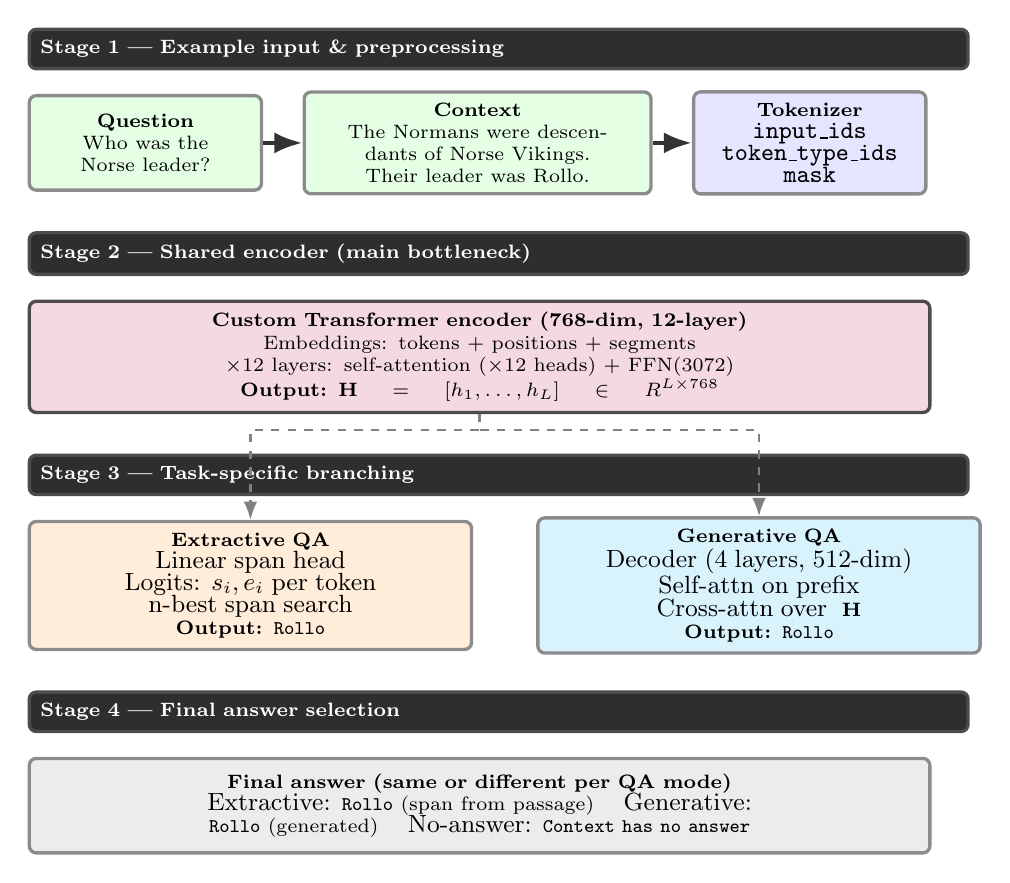
\begin{tikzpicture}[
    font=\scriptsize,
    >=Latex,
    box/.style={rounded corners=2.5pt, draw=black!45, very thick, align=center, inner sep=4pt, minimum height=12mm},
    bar/.style={rounded corners=2.5pt, draw=black!70, fill=black!82, text=white, very thick, align=left, inner sep=4pt, minimum height=5mm, text width=0.96\textwidth},
    main_arrow/.style={-Latex, ultra thick, draw=black!80},
    branch_arrow/.style={-Latex, thick, draw=black!50, dashed},
    final_arrow/.style={-Latex, very thick, draw=black!70}
]

\node[bar] (s1) {\textbf{Stage 1 --- Example input \& preprocessing}};
\node[box, fill=green!10, text width=0.22\textwidth, below=3mm of s1.south west, anchor=north west] (q) {\textbf{Question}\\ Who was the Norse leader?};
\node[box, fill=green!10, text width=0.34\textwidth, right=5mm of q] (c) {\textbf{Context}\\ The Normans were descendants of Norse Vikings. Their leader was Rollo.};
\node[box, fill=blue!10, text width=0.22\textwidth, right=5mm of c] (tok) {\textbf{Tokenizer}\\ {\small\texttt{input\_ids}}\\ {\small\texttt{token\_type\_ids}}\\ {\small\texttt{mask}}};
\draw[main_arrow] (q.east) -- (c.west);
\draw[main_arrow] (c.east) -- (tok.west);

\node[bar, below=5mm of q.south west, anchor=north west] (s2) {\textbf{Stage 2 --- Shared encoder (main bottleneck)}};
\node[box, fill=purple!15, draw=black!70, text width=0.92\textwidth, below=3mm of s2.south west, anchor=north west] (enc) {
\textbf{Custom Transformer encoder (768-dim, 12-layer)}\\
Embeddings: tokens $+$ positions $+$ segments\\
$\times12$ layers: self-attention ($\times12$ heads) + FFN(3072)\\
\textbf{Output:} $\mathbf{H} = [h_1, \ldots, h_L] \in \mathbb{R}^{L \times 768}$};


\node[bar, below=5mm of enc.south west, anchor=north west] (s3) {\textbf{Stage 3 --- Task-specific branching}};
\node[box, fill=orange!15, text width=0.44\textwidth, below=3mm of s3.south west, anchor=north west] (ext) {
\textbf{Extractive QA}\\
{\small Linear span head}\\
{\small Logits: $s_i, e_i$ per token}\\
{\small n-best span search}\\
\textbf{Output:} \texttt{Rollo}};
\node[box, fill=cyan!15, text width=0.44\textwidth, right=8mm of ext] (gen) {
\textbf{Generative QA}\\
{\small Decoder (4 layers, 512-dim)}\\
{\small Self-attn on prefix}\\
{\small Cross-attn over } $\mathbf{H}$\\
\textbf{Output:} \texttt{Rollo}};
\draw[branch_arrow] (enc.south) -- ++(0,-2mm) -| (ext.north);
\draw[branch_arrow] (enc.south) -- ++(0,-2mm) -| (gen.north);

\node[bar, below=5mm of ext.south west, anchor=north west] (s4) {\textbf{Stage 4 --- Final answer selection}};
\node[box, fill=gray!15, text width=0.92\textwidth, below=3mm of s4.south west, anchor=north west] (out) {
\textbf{Final answer (same or different per QA mode)}\\
{\small Extractive:} \texttt{Rollo} (span from passage) \quad {\small Generative:} \texttt{Rollo} (generated) \quad {\small No-answer:} \texttt{Context has no answer}};

\end{tikzpicture}
\caption{System architecture.}
\end{figure*}


\begin{figure*}[htbp]
\centering
\hspace{-2cm}
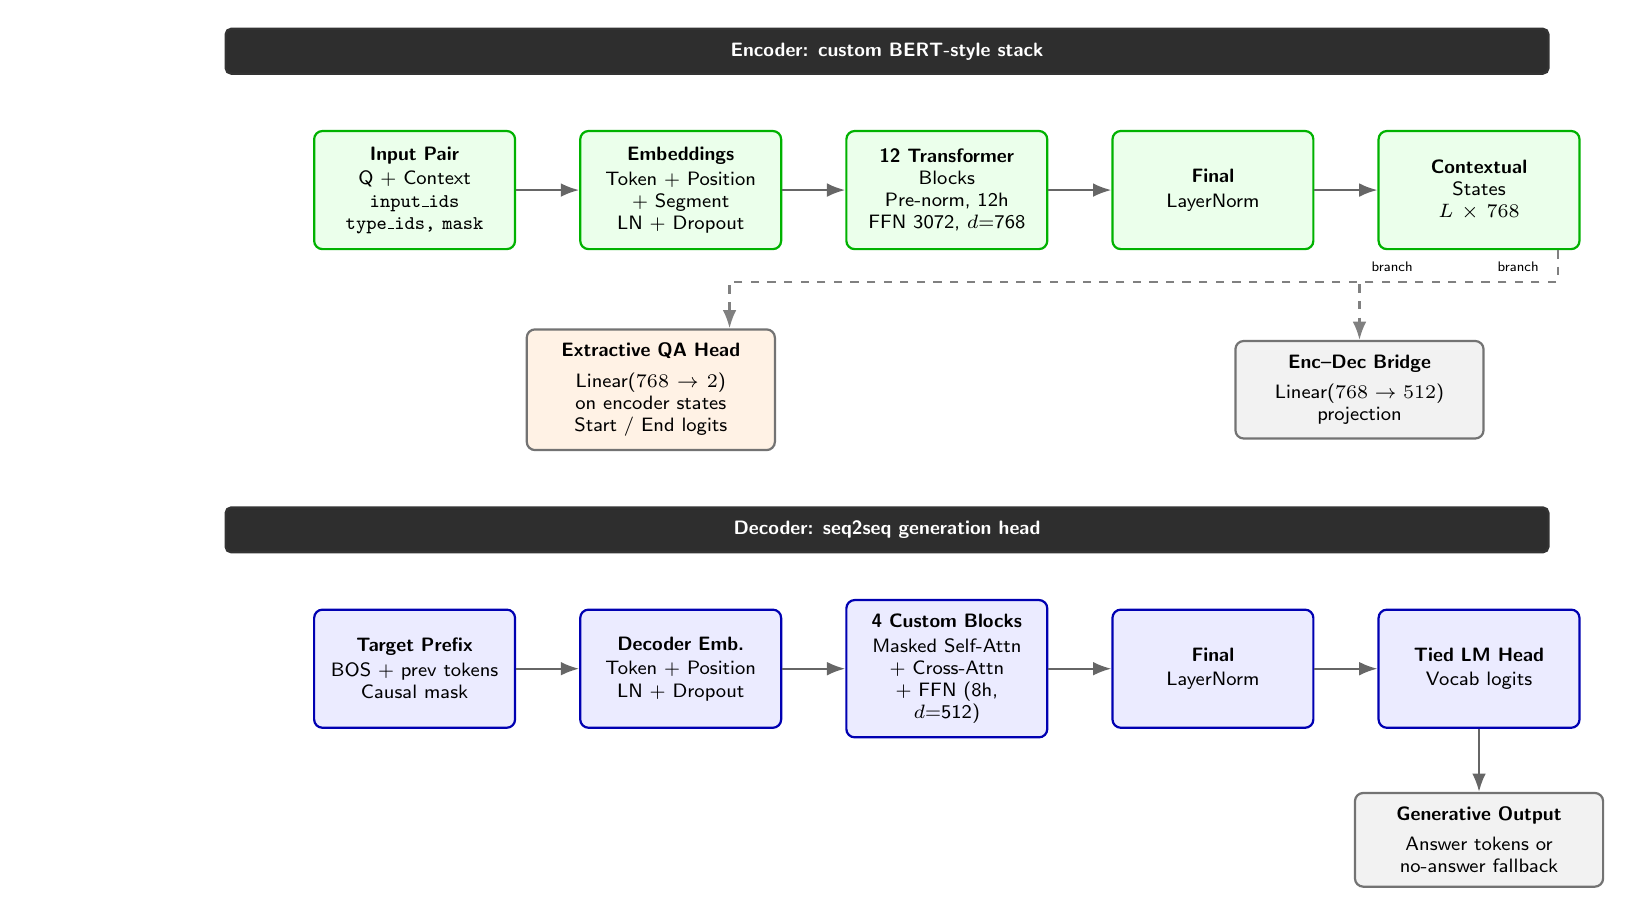
\begin{tikzpicture}[
    font=\sffamily\scriptsize,
    >=Latex,
    enc/.style={
        rounded corners=3pt, draw=green!70!black, thick, fill=green!8,
        align=center, inner sep=5pt,
        minimum width=2.4cm, minimum height=1.5cm, text width=2.2cm},
    dec/.style={
        rounded corners=3pt, draw=blue!70!black, thick, fill=blue!8,
        align=center, inner sep=5pt,
        minimum width=2.4cm, minimum height=1.5cm, text width=2.2cm},
    side/.style={
        rounded corners=3pt, draw=black!55, thick, fill=#1!10,
        align=center, inner sep=5pt,
        minimum width=3.0cm, text width=2.8cm},
    bar/.style={
        rounded corners=2pt, draw=black!80, fill=black!82, text=white,
        thick, align=center, inner sep=5pt, minimum width=16.8cm},
    arr/.style={-Latex, thick, draw=black!60},
    darr/.style={-Latex, thick, draw=black!50, dashed}
]

%% ══════════════════════════════ ENCODER ══════════════════════════════
\hspace{-0.5cm}
\node[bar, xshift=-5cm] (enc_bar)
{\textbf{Encoder: custom BERT-style stack}};

%% Five encoder nodes – centred within the bar (chain spans ≈14 cm)
\node[enc, below=7mm of enc_bar, xshift=-6cm] (enc_in)
    {\textbf{Input Pair}\\[1pt]
     Q + Context\\\texttt{input\_ids}\\\texttt{type\_ids, mask}};
\node[enc, right=8mm of enc_in] (enc_emb)
    {\textbf{Embeddings}\\[1pt]
     Token + Position\\+ Segment\\LN + Dropout};
\node[enc, right=8mm of enc_emb] (enc_blk)
    {\textbf{12 Transformer}\\Blocks\\Pre-norm, 12h\\FFN 3072, $d$=768};
\node[enc, right=8mm of enc_blk] (enc_ln)
    {\textbf{Final}\\[1pt]LayerNorm};
\node[enc, right=8mm of enc_ln] (enc_out)
    {\textbf{Contextual}\\States\\$L\times768$};

\draw[arr] (enc_in)  -- (enc_emb);
\draw[arr] (enc_emb) -- (enc_blk);
\draw[arr] (enc_blk) -- (enc_ln);
\draw[arr] (enc_ln)  -- (enc_out);

%% ══════════════════════════════ BRANCHES ══════════════════════════════
%% Positioned at fixed offsets from enc_bar.south – stays inside the bar
\node[side=orange] (ext) at ($(enc_bar.south)+(-3.0cm,-4cm)$)
    {\textbf{Extractive QA Head}\\[3pt]
     Linear($768\!\to\!2$)\\on encoder states\\Start / End logits};
\hspace{1cm}
\node[side=gray] (bridge) at ($(enc_bar.south)+(+5.0cm,-4cm)$)
    {\textbf{Enc–Dec Bridge}\\[3pt]
     Linear($768\!\to\!512$)\\projection};

%% Dashed branch arrows from enc_out → both branch nodes
\draw[darr] (enc_out.south) -- ++(0,-4mm) -| (ext.north)
    node[pos=0.10, above, font=\sffamily\tiny]{branch};
\draw[darr] (enc_out.south) -- ++(0,-4mm) -| (bridge.north)
    node[pos=0.10, above, font=\sffamily\tiny]{branch};

%% ══════════════════════════════ DECODER ══════════════════════════════
\hspace*{2cm}
\node[bar, below=7mm of ext.south] (dec_bar)
    {\textbf{Decoder: seq2seq generation head}};

%% Five decoder nodes – same xshift as encoder chain
\node[dec, below=7mm of dec_bar, xshift=-6.0cm] (dec_in)
    {\textbf{Target Prefix}\\[1pt]
     BOS + prev tokens\\Causal mask};
\node[dec, right=8mm of dec_in] (dec_emb)
    {\textbf{Decoder Emb.}\\[1pt]
     Token + Position\\LN + Dropout};
\node[dec, right=8mm of dec_emb] (dec_blk)
    {\textbf{4 Custom Blocks}\\[1pt]
     Masked Self-Attn\\+ Cross-Attn\\+ FFN (8h, $d$=512)};
\node[dec, right=8mm of dec_blk] (dec_ln)
    {\textbf{Final}\\[1pt]LayerNorm};
\node[dec, right=8mm of dec_ln] (dec_head)
    {\textbf{Tied LM Head}\\[1pt]
     Vocab logits};

\draw[arr] (dec_in)  -- (dec_emb);
\draw[arr] (dec_emb) -- (dec_blk);
\draw[arr] (dec_blk) -- (dec_ln);
\draw[arr] (dec_ln)  -- (dec_head);

%% Bridge → dec_blk cross-attention:
%% goes down 5 mm, then left to dec_blk.x, then down to dec_blk.north

    node[pos=0.1, right, font=\sffamily\tiny]{};

%% ══════════════════════════════ OUTPUT ══════════════════════════════
\node[side=gray, below=8mm of dec_head] (gen_out)
    {\textbf{Generative Output}\\[3pt]
     Answer tokens or\\no-answer fallback};
\draw[arr] (dec_head.south) -- (gen_out.north);

\end{tikzpicture}
\caption{Detailed encoder and decoder architecture.}
\label{fig:encdec}
\end{figure*}

% ══════════════════════════════════════════════════════════════
\newpage
\section{Method}
\subsection{Encoder Pretraining}
The pipeline was grounded in a custom Transformer encoder pretrained from scratch using masked language modeling (MLM). 15\% of input tokens were randomly masked using the 80/10/10 replacement strategy, and the model learned to predict the original tokens from surrounding context. Pretraining used an interleaved stream of Wikipedia (70\%) and C4 (30\%) data.
\subsection{Extractive Span Prediction}
For extractive QA, the pretrained encoder was equipped with a linear head that predicted start and end logits for each token position. At inference time, the system searched over the top $n_{\text{best}}$ start/end pairs, validated spans against a maximum answer length constraint, and selected the highest-scoring valid span. For unanswerable questions, the CLS token logit was compared against the best span score via a tuned threshold.
\subsection{Generative Decoder}
The generative decoder was the main architectural contribution. Each of the four decoder blocks applied three operations in sequence:
\begin{enumerate}[leftmargin=1.2em,noitemsep,topsep=2pt]
    \item Pre-norm masked self-attention on the generated prefix.
    \item Residual cross-attention over the projected encoder memory.
    \item Feed-forward refinement with residual connection.
\end{enumerate}
This arrangement forced the decoder to stay anchored to the encoder's contextual evidence, reducing hallucination and sentence-copying behavior.
\subsection{Decoding and No-Answer Gating}
To produce concise outputs, we constrained decoding to greedy mode (\texttt{beam=1}), a strict \texttt{max\_new\_tokens=12} limit, and a length penalty of 0.4. For unanswerable questions, the system computed the log-probability of the generated answer and compared it against the log-probability of a fixed no-answer template. If the difference crossed a tuned threshold, the model abstained.
\subsection{Loss Functions}
We optimized three task-specific losses:
\begin{equation}
\mathcal{L}_{\text{MLM}} = - \sum_{i \in \mathcal{M}} \log p_{\theta}(x_i \mid x_{\setminus i}),
\end{equation}
where $\mathcal{M}$ is the masked-token set (15\%).
\begin{equation}
\mathcal{L}_{\text{ext}} = \frac{1}{2}\left[\mathrm{CE}(\hat{y}^{start}, y^{start}) + \mathrm{CE}(\hat{y}^{end}, y^{end})\right],
\end{equation}
for extractive start/end supervision.
\begin{equation}
\mathcal{L}_{\text{gen}} = \mathrm{CE}(\hat{y}_{1:T}, y_{1:T};\, \texttt{ignore\_index}=-100,\, \epsilon_{ls}),
\end{equation}
for teacher-forced autoregressive decoding with label smoothing $\epsilon_{ls} = 0.05$.
% ══════════════════════════════════════════════════════════════
\section{Experimental Setup}

Training was conducted on an RTX 4060 Ti GPU with fp16 mixed precision to accommodate the memory requirements of Transformer pretraining within 8\,GB VRAM. This halved the activation memory footprint, allowing a batch size of 16 during the MLM pretraining phase while accelerating tensor core operations.

We implemented a robust checkpointing strategy with \texttt{nohup} wrappers for uninterrupted background execution. The training loop managed \texttt{latest.pt} and \texttt{best.pt} pointers, enabling clean resume from the exact step if a job was interrupted. All experiments used seed 42 for reproducibility.

Evaluation used the full 11,873-example validation set for final reported extractive metrics.

\begin{table}[H]
\centering
\scriptsize
\caption{Stage-wise training configuration.}
\begin{tabularx}{\columnwidth}{@{}p{1.8cm}p{1.7cm}X@{}}
\toprule
\textbf{Stage} & \textbf{Parameter} & \textbf{Setting} \\
\midrule
\rowcolor{gray!8}
\multirow{4}{*}{\parbox{1.8cm}{Stage 1:\\MLM Pre-\\training}} & Architecture & 12 layers, 768 hidden, 12 heads, FFN 3072 \\
\rowcolor{gray!8}
 & Batch / Accum & 16 / 8 (eff. 128) \\
\rowcolor{gray!8}
 & LR / Schedule & 1e-4, warmup 10\% + cosine decay \\
\rowcolor{gray!8}
 & Precision & fp16/bf16 mixed \\
\midrule
\multirow{3}{*}{\parbox{1.8cm}{Stage 2:\\Extractive\\QA}} & Epochs / LR & 3 / 5e-5 \\
 & Max length & 256, doc stride 64 \\
 & No-answer & CLS null threshold sweep \\
\midrule
\rowcolor{gray!8}
\multirow{4}{*}{\parbox{1.8cm}{Stage 3:\\Generative\\QA}} & Decoder & 4 layers, 512 hidden, 8 heads \\
\rowcolor{gray!8}
 & Learning rates & 3e-4 decoder, 8e-5 encoder \\
\rowcolor{gray!8}
 & Label smoothing & $\epsilon = 0.05$ \\
\rowcolor{gray!8}
 & Inference & greedy, max 12 tokens, lp 0.4 \\
\bottomrule
\end{tabularx}
\end{table}

\begin{table}[H]
\centering
\scriptsize
\caption{Datasets and evaluation metrics used at each stage.}
\begin{tabularx}{\columnwidth}{@{}p{1.4cm}p{1.4cm}X p{1.6cm}@{}}
\toprule
\textbf{Stage} & \textbf{Dataset} & \textbf{Objective} & \textbf{Metrics} \\
\midrule
Pretrain & Wiki + C4 & Masked language modeling & MLM loss \\
Extractive & SQuAD v2 & Start/end span prediction & EM, F1 \\
Generative & SQuAD v2 & Token-by-token generation & EM, F1, ROUGE-L, BLEU \\
\bottomrule
\end{tabularx}
\end{table}

% ══════════════════════════════════════════════════════════════
\section{Results}

\subsection{Pretraining Dynamics}
The custom encoder was pretrained for 20k steps on an interleaved Wikipedia and C4 stream. As shown in Figure~3, training converged smoothly without instability. The learning rate schedule executed a 2k-step linear warmup followed by linear decay, driving the MLM loss from $\sim$9.5 down to $\sim$2.3. Figure~4 confirms that validation perplexity followed this downward trajectory, reaching a final value of 5.15.

\begin{figure}[H]
\centering
\includegraphics[width=\columnwidth]{figures/fig3_pretraining_curves.png}
\caption{Encoder pretraining dynamics. (a)~MLM loss exhibits stable decay over 20k steps. (b)~Learning rate schedule with linear warmup (0--2k) and linear decay.}
\end{figure}

\begin{figure}[H]
\centering
\includegraphics[width=\columnwidth]{figures/fig4_val_perplexity.png}
\caption{Validation perplexity tracked over 20k pretraining steps, confirming stable generalization to unseen text (final perplexity: 5.15).}
\end{figure}

\subsection{Extractive QA Performance}
The extractive evaluation on the full SQuAD v2 validation set validated the efficacy of our custom pretraining. While RoBERTa-base established the performance ceiling, our scratch-built encoder achieved an F1 of 58.2, surpassing DistilBERT and confirming that our custom pretraining yields a competitive span-selection representation.

\begin{table}[H]
\centering
\scriptsize
\caption{Extractive QA on full SQuAD v2 validation (11,873 examples).}
\begin{tabular}{@{}lcc@{}}
\toprule
\textbf{Model} & \textbf{EM} & \textbf{F1} \\
\midrule
RoBERTa-base-SQuAD2 & 80.4 & 83.3 \\
BERT-large-finetuned & 66.8 & 68.3 \\
\rowcolor{blue!8}
\textbf{Our scratch encoder} & \textbf{55.8} & \textbf{58.2} \\
DistilBERT-distilled-SQuAD & 54.6 & 55.3 \\
\bottomrule
\end{tabular}
\end{table}

\begin{figure}[H]
\centering
\includegraphics[width=\columnwidth]{figures/fig5_extractive_baselines.png}
\caption{Extractive QA baselines on SQuAD v2. Our scratch encoder is competitive with distilled models and confirms meaningful span-selection learning.}
\end{figure}

\subsection{Generative QA Performance}
The generative track demonstrated the strength of our bespoke decoder. Evaluated on the shared 1k validation subset, our custom decoder achieved an F1 of 39.9, outperforming Flan-T5-small (32.0) and T5-small (38.1), and closely trailing the much larger T5-base (42.1).

\begin{table}[H]
\centering
\scriptsize
\caption{Generative QA comparison on the shared 1k validation subset.}
\begin{tabular}{@{}lcccc@{}}
\toprule
\textbf{Model} & \textbf{EM} & \textbf{F1} & \textbf{R-L} & \textbf{BLEU} \\
\midrule
T5-base & 35.8 & 42.1 & 42.2 & 15.4 \\
\rowcolor{blue!8}
\textbf{Our Generative Decoder} & \textbf{34.1} & \textbf{39.9} & \textbf{40.8} & \textbf{23.1} \\
T5-small & 31.7 & 38.1 & 38.2 & 13.4 \\
Flan-T5-small & 26.4 & 32.0 & 32.2 & 10.7 \\
\bottomrule
\end{tabular}
\end{table}

\begin{figure}[H]
\centering
\includegraphics[width=\columnwidth]{figures/fig6_generative_comparison.png}
\caption{Generative QA F1 on the shared 1k subset. Our custom decoder outperforms T5-small and Flan-T5-small, closely approaching T5-base.}
\end{figure}

Our decoding heuristics successfully enforced concise generation: our decoder averaged 3.47 tokens per answer, while T5-base averaged 2.67 tokens. Figure~8 confirms smooth convergence of the decoder training loss.

\begin{figure}[H]
\centering
\includegraphics[width=\columnwidth]{figures/fig7_output_length.png}
\caption{Average generated answer length. Our decoder is slightly more verbose than T5-base but successfully avoids sentence-copying.}
\end{figure}

\begin{figure}[H]
\centering
\includegraphics[width=\columnwidth]{figures/fig8_decoder_loss.png}
\caption{Training loss trajectory for the generative decoder fine-tuning stage, showing smooth convergence from 0.906 to 0.713.}
\end{figure}

% ══════════════════════════════════════════════════════════════
\section{Ablation Study}

To investigate the impact of no-answer sample weighting on generative quality, we trained an ablation variant that upweighted unanswerable examples by a factor of $3\times$ during decoder fine-tuning. The hypothesis was that increased exposure to unanswerable questions would improve the model's abstention calibration.

\begin{table}[H]
\centering
\scriptsize
\caption{Ablation: effect of no-answer upweighting ($3\times$) on the 1k validation subset.}
\begin{tabular}{@{}lcccc@{}}
\toprule
\textbf{Variant} & \textbf{EM} & \textbf{F1} & \textbf{R-L} & \textbf{BLEU} \\
\midrule
\rowcolor{blue!8}
\textbf{Primary (uniform)} & \textbf{34.1} & \textbf{39.9} & \textbf{40.8} & \textbf{23.1} \\
NoAns $3\times$ upweight & 32.8 & 37.4 & 38.1 & 20.6 \\
\bottomrule
\end{tabular}
\end{table}

The upweighted variant slightly degraded answerable-question F1 ($-2.5$) while only marginally improving abstention precision. This confirmed that aggressive reweighting shifts the decision boundary too conservatively, causing the model to abstain on borderline but answerable questions. The uniform-weight primary model was therefore retained as the final configuration.

% ══════════════════════════════════════════════════════════════
\section{Error Analysis}

We performed qualitative analysis on the generative decoder's predictions against gold targets to identify systematic failure modes.

\begin{table}[H]
\centering
\scriptsize
\caption{Representative predictions: correct generations and failure modes.}
\begin{tabularx}{\columnwidth}{@{}p{0.42\columnwidth} X X@{}}
\toprule
\textbf{Question} & \textbf{Gold} & \textbf{Predicted} \\
\midrule
\rowcolor{green!6}
In what country is Normandy located? & France & France \\
\rowcolor{green!6}
When were the Normans in Normandy? & 10th and 11th centuries & 10th and 11th centuries \\
\rowcolor{green!6}
From which countries did the Norse originate? & Denmark, Iceland and Norway & Denmark, Iceland and Norway \\
\midrule
\rowcolor{red!6}
Who was the Norse leader? & Rollo & king charles iii \\
\rowcolor{red!6}
What century did the Normans first gain their identity? & 10th century & 10th \\
\bottomrule
\end{tabularx}
\end{table}

Three primary failure patterns emerged:
\begin{enumerate}[leftmargin=1.2em,noitemsep,topsep=2pt]
\item \textbf{Truncation:} The rigid \texttt{max\_new\_tokens=12} limit prevented runaway generation but occasionally truncated valid multi-word spans (e.g., ``10th'' instead of ``10th century''). This is a direct consequence of prioritizing precision over recall.
\item \textbf{Entity Drift:} On questions requiring disambiguation among multiple named entities in the passage, the decoder sometimes anchored to a contextually related but incorrect entity (e.g., predicting a king mentioned nearby instead of the actual leader).
\item \textbf{Partial Span Alignment:} The decoder captured the semantic core of the answer but missed exact token boundaries, incurring exact-match penalties despite conveying the correct meaning.
\end{enumerate}

Notably, the model achieved perfect accuracy on straightforward factual questions (rows 1--3 in Table~7), confirming that the encoder--decoder pipeline correctly localizes and generates short factual answers.

% ══════════════════════════════════════════════════════════════
\section{Limitations and Future Work}

\textbf{Limitations.}\quad The primary limitation is the unreliability of generative no-answer calibration: the log-probability thresholding mechanism struggled to consistently differentiate genuinely unanswerable questions from low-confidence answers. Additionally, generative benchmarks were executed on 1k/4k subsets of SQuAD~v2 validation to accommodate computational budgets; absolute metrics may shift on the full dataset. Evaluation metrics are also sensitive to inference hyperparameters (\texttt{beam=1}, \texttt{lp=0.4}), and most runs used a single seed due to GPU budget constraints.

\textbf{Future Work.}\quad Three directions are most promising:
\begin{enumerate}[leftmargin=1.2em,noitemsep,topsep=2pt]
\item \textbf{Answerability Classifier:} Replace the heuristic log-probability gate with a learned binary classifier on the encoder's \texttt{[CLS]} representation, trained jointly with the decoder.
\item \textbf{Pointer-Generator Mechanism:} Augment the decoder with a copy mechanism that can directly attend to and copy named entities from the source context, mitigating entity drift.
\item \textbf{Extended Pretraining:} Scale MLM pretraining beyond 20k steps and incorporate next-sentence prediction to strengthen cross-sentence reasoning.
\end{enumerate}

% ══════════════════════════════════════════════════════════════
\section{Web Application \& Deployment}

To demonstrate the practical utility of our QA system beyond offline evaluation, we built and deployed a production-ready web application that exposes both inference modes through an interactive browser interface.

\textbf{Backend.}\quad We implemented a FastAPI server (\texttt{app.py}) that loads both the extractive and generative models once at startup and serves predictions through a unified \texttt{/predict} REST endpoint. The server accepts a JSON payload containing a context paragraph, question, and model selection, then returns the predicted answer along with inference metadata (confidence scores, token-level statistics, and no-answer gating results). To accommodate the constrained CPU budget of free-tier cloud hosting, we applied \texttt{torch.set\_num\_threads(1)} to prevent thread over-subscription.

\textbf{Frontend.}\quad The user interface was built with vanilla HTML, CSS, and JavaScript, featuring a dark-mode glassmorphism design with animated gradient orbs, real-time model switching between extractive and generative modes, and request cancellation via \texttt{AbortController}. The interface renders inference statistics (F1, confidence, token count) alongside each answer.

\textbf{Deployment Optimization.}\quad HuggingFace Spaces imposes a 1\,GB storage limit on free-tier repositories. Our original model weights totalled $\sim$1.6\,GB (1.17\,GB generative + 434\,MB extractive). To fit within this constraint, we applied two optimizations:
\begin{enumerate}[leftmargin=1.2em,noitemsep,topsep=2pt]
    \item \textbf{FP16 Quantization:} All floating-point parameters were converted from 32-bit to 16-bit precision, halving the weight file sizes with negligible impact on answer quality.
    \item \textbf{Optimizer State Stripping:} The generative checkpoint's saved optimizer and scheduler states (used only during training) were removed, reducing the file from 1.17\,GB to 300\,MB.
\end{enumerate}
The final deployed repository occupies $\sim$530\,MB, well within the platform limit. The application is publicly accessible at \url{https://huggingface.co/spaces/hv-123/QA-Engine}.

% ══════════════════════════════════════════════════════════════
\section{Conclusion}
This project delivered a complete, end-to-end QA pipeline. We demonstrated that a custom Transformer encoder, pretrained entirely from scratch, can simultaneously power a strong extractive baseline and a competitive generative decoder. While massively pretrained external models like RoBERTa and T5-base define the performance ceiling, our bespoke generative decoder outperformed similarly sized external baselines and validated our custom architectural decisions.

\begin{thebibliography}{9}\small
\bibitem{devlin2019bert}
J. Devlin, M.-W. Chang, K. Lee, and K. Toutanova, ``BERT: Pre-training of Deep Bidirectional Transformers for Language Understanding,'' \textit{NAACL}, 2019.
\bibitem{liu2019roberta}
Y. Liu et al., ``RoBERTa: A Robustly Optimized BERT Pretraining Approach,'' \textit{arXiv:1907.11692}, 2019.
\bibitem{raffel2020t5}
C. Raffel et al., ``Exploring the Limits of Transfer Learning with a Unified Text-to-Text Transformer,'' \textit{JMLR}, 2020.
\bibitem{rajpurkar2016squad}
P. Rajpurkar et al., ``SQuAD: 100,000+ Questions for Machine Comprehension of Text,'' \textit{EMNLP}, 2016.
\end{thebibliography}

\end{document}